\documentclass{beamer}
% Für schnelleres Kompilieren:
%\documentclass[draft]{beamer}
%\includeonlyframes{toc,current}

\mode<presentation>
{
  \usetheme{Malmoe}
  % Antibes, Pittsburgh, Dresden, Berlin, Goettingen, Luebeck, Rochester
  \setbeamercovered{transparent}
}

\usepackage{listings}

\definecolor{hellgelb}{rgb}{1,1,0.8}
\definecolor{hellgrau}{rgb}{0.95,0.95,0.95}
\definecolor{colKeys}{rgb}{0,0,1}
\definecolor{colIdentifier}{rgb}{0,0,0}
\definecolor{colComments}{rgb}{0.7,0.7,0.7}
\definecolor{colString}{rgb}{0,0.5,0}

%%% Konfiguration des listing-Paketes
\lstset{%
	float=hbp,%
	identifierstyle=\color{colIdentifier}, %
	basicstyle=\ttfamily\scriptsize,%
	stringstyle=\ttfamily,%
	keywordstyle=\color{colKeys}, %
	stringstyle=\color{colString}, %
	commentstyle=\color{colComments}, %
	columns=flexible, %
	tabsize=2, %
% 	frame=tb, %
	extendedchars=true, %
	showspaces=false, %
	showstringspaces=false, %
	numbers=left, %
	numberstyle=\tiny, %
	breaklines=true, %
	backgroundcolor=\color{hellgelb}, %
	breakautoindent=true, %
	captionpos=b%,
% 	aboveskip=\bigskipamount,%
% 	belowskip=\medskipamount,%
	escapeinside={(*}{*)}, %
% 	mathescape, %
	language=oz
}

\usepackage[german]{babel}
\usepackage[utf8]{inputenc}
\usepackage[T1]{fontenc}
\usepackage{lmodern}
%\usepackage{times}
\usepackage{multimedia}

\title[WBSY SS07]{The Mozart Programming System}
\author[Ruf, Tammen]{Tobias Ruf, Jan Tammen}

\institute{
  Wissensbasierte Systeme SS 07,\\
  Fakultät Informatik,\\
  HTWG Konstanz
}

%%% Informationen ueber das PDF-Dokument setzen
\hypersetup{
  pdftitle={The Mozart Programming System},%
  pdfauthor={Jan Tammen,%
  			 Tobias Ruf},%
  pdfsubject={Wissensbasierte Systeme},%
  pdfcreator={LaTeX with pdfeTeX},%
  pdfproducer={LaTeX with pdfeTeX},%
  pdfkeywords={<Keywords>},
  % pdfpagelayout=TwoColumnRight,
  pdffitwindow=true,
  pdfpagemode=FullScreen,
%  pdfstartview=FitH,
}

\date{24.~April 2007}
\subject{The Mozart Programming Systeme}

\pgfdeclareimage[height=1cm]{htwg-logo}{../images/htwg-logo}
\logo{\pgfuseimage{htwg-logo}}

% Folgendes sollte gelöscht werden, wenn man nicht am Anfang jedes
% Unterabschnitts die Gliederung nochmal sehen möchte.
\AtBeginSection[]
{
 \begin{frame}<beamer>
   %\frametitle{Gliederung}
   \tableofcontents[currentsection,currentsubsection]
 \end{frame}
}

% Falls Aufzählungen immer schrittweise gezeigt werden sollen, kann
% folgendes Kommando benutzt werden:
% mit highlight: <+- | alert@+>
%\beamerdefaultoverlayspecification{<+->}

\begin{document}

% Frame: Titelseite
\begin{frame}
  \centering\pgfimage[width=0.5\textwidth]{../images/mozart-logo}
  \titlepage
\end{frame}

% Frame: Gliederung
\begin{frame}[label=toc]
  \tableofcontents
\end{frame} 

\section{Einleitung}
\section{The Mozart Programming System}
In der vorliegenden Ausarbeitung soll das "`Mozart Programming System"'
\footnote{\url{http://www.mozart-oz.org}} 
vorgestellt werden. Bei \textsl{Mozart} handelt es sich um eine 
Programmierumgebung, die die multiparadigmische Programmiersprache \textsl{Oz} 
implementiert.

Entstanden ist Mozart-Oz ursprünglich als Forschungsprojekt am Deutschen 
Forschungszentrum für Künstliche Intelligenz (DFKI) sowie der Universität 
Saarbrücken. Inzwischen wird die Sprache vom Mozart-Konsortium, zu welchem 
Arbeitsgruppen aus Belgien, Schweden und Deutschland gehören, weiterentwickelt. 
Die Quellen sind unter einer Open-Source-Lizenz verfügbar; ein kommerzieller 
Einsatz der Sprache ist ebenfalls möglich.

Ähnlich wie in Java können Oz-Programme in eine Art Byte-Code übersetzt werden 
und laufen anschließend in einer virtuellen Maschine ab. Auf diese Weise wird 
eine gewisse Plattformunabhängigkeit erreicht.

\section{Die Programmiersprache Oz}
\subsection{Features}
Als Hauptfeatures und -vorteile von Oz gelten die folgenden Aspekte:

\begin{description}
  \item[Nebenläufigkeit] Arbeit mit leichtgewichtigen Threads, 
  Datenfluss-Synchronisation.
  \item[Inferencing] Constraintbasierte und 
  logische Programmierung.
  \item[Verteilung] Transparente 
  Netzwerkunterstützung.
  \item[Flexibilität] Dynamische Typisierung, inkrementelles 
  Kompilieren.
\end{description}

\subsection{Datentypen}
Die Sprache stellt eine Reihe von Datentypen zur Verfügung, deren Hierarchie in 
Abbildung \ref{fig:oz-datentypen} dargestellt ist.

\begin{figure}[hp]
  \centering 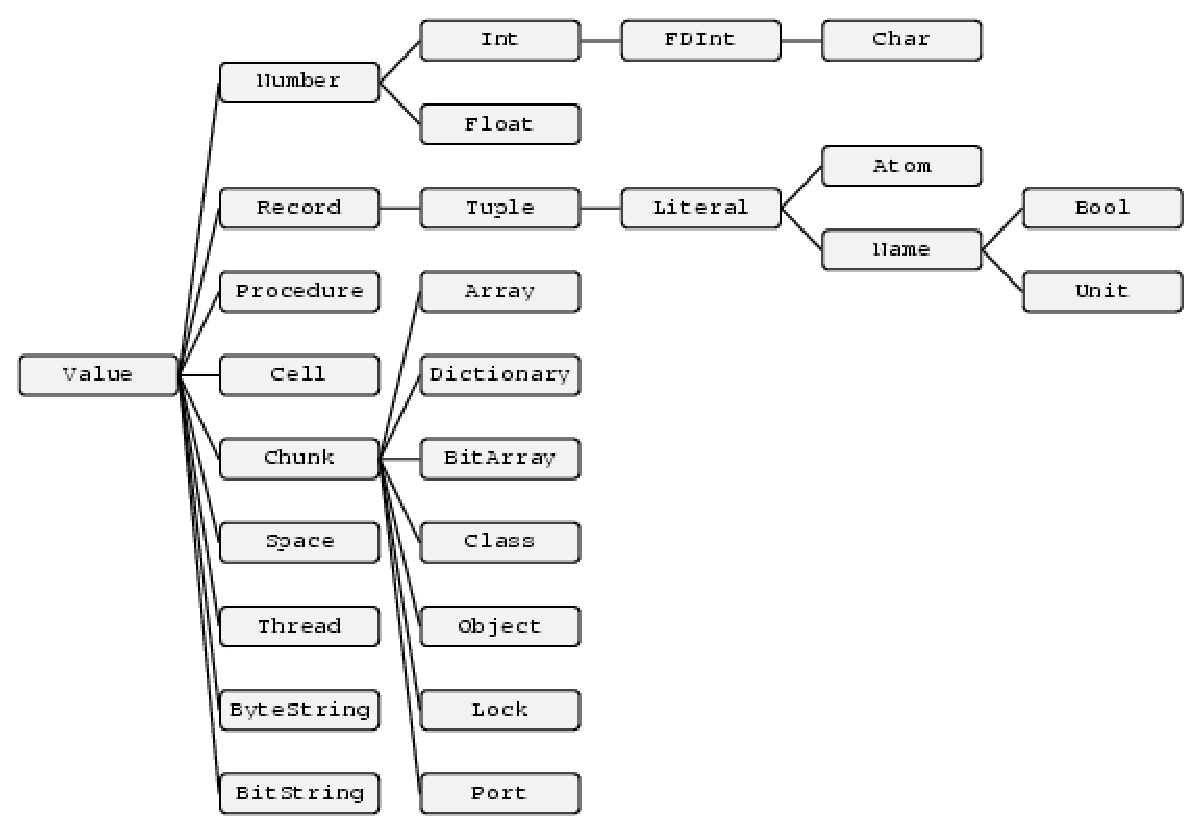
\includegraphics[width=0.70\textwidth]{../images/oz-datentypen} 
  \caption{Hierarchie der Datentypen in Oz 3. Quelle:
  \cite[Tutorial of Oz, Chapter 3.1]{url:mozart-documentation}}
  \label{fig:oz-datentypen}
\end{figure}

Einige der wichtigsten Datentypen seien hier kurz aufgeführt (vgl. 
\cite{Brunklaus:00}).

\begin{enumerate}
  \item Einfache Werte
    \begin{description}
      \item [Zahlen] können in Oz sowohl als ganze Zahlen (\texttt{Int, Char})
      als auch Fließkommazahlen (\texttt{Float}) benutzt werden.
      \item[Literale] teilen sich auf in sog. Atome und Namen. Ein Atom wird 
      durch eine alphanumerische Zeichenkette beschrieben, die entweder mit 
      einem Kleinbuchstaben beginnt oder in Hochkomma gefasst ist. Namen sind 
      eindeutige Bezeichner, die über eine spezielle Prozedur namens 
      \texttt{NewName} erzeugt werden können.
      \item[Prozeduren] können in Oz an Variablen gebunden und auch zur 
      Laufzeit erzeugt werden. \end{description}
  \item Zusammengesetzte Werte
    \begin{description}
      \item[Records] bestehen aus einem Bezeichner (Label) sowie einer festen 
      Anzahl von Komponenten oder Argumenten. Argumente bestehen aus dem Tupel 
      (Feature, Feld).
      \item[Tupel] sind ein Spezialfall von Records, bei denen die Argumente 
      kein explizites Feature besitzen.
      \item[Listen] sind eine Sonderform der Tupel. Die leere Liste wird mit
      \texttt{nil} denotiert, offene Listen bspw. als \texttt{1|2|3|nil} und 
      geschlossene Listen (also Listen mit fester Elementanzahl) als \texttt{[1 
      2 3]}.
    \end{description}
  \item \textbf{Chunks} erlauben es, abstrakte Datentypen zu konstruieren. 
  Oz bringt bereits einige vordefinierte Chunks mit, z.B. \texttt{Array} 
  oder \texttt{Dictionary}.
\end{enumerate}

\subsection{Multiparadigmisch?}
Wie bereits eingangs erwähnt, unterstützt Oz mehrere Programmierparadigmen:

\begin{enumerate}
  \item Constraint-Programmierung
  \item Funktionale Programmierung
  \item Objektorientierte Programmierung
  \item Logische Programmierung
\end{enumerate}
  
Im Gegensatz zu einer Programmiersprache, die nur eines der Paradigmen 
unterstützt, lassen sich in Oz also die zu lösenden Probleme von mehreren 
Seiten gleichzeitig mit dem jeweils geeignetsten Paradigma bearbeiten. 
Erreichen könnte man dies zwar auch durch die Kombination verschiedener 
Programmiersprachen, dabei bliebe aber der Nachteil, dass man semantische 
Lücken überwinden und Schnittstellen zwischen den einzelnen Sprachen definieren 
müsste. Dies würde u.a. zu einer aufwendigeren Fehlersuche führen. Mit Oz 
lassen sich hingegen die verschiedene Paradigmen problemlos miteinander 
kombinieren, deren gemeinsame Basis, das Oz Programming Model, im nächsten 
Abschnitt vorgestellt wird.

\subsection{Programmiermodell (Oz Programming Model, OPM)}
Die Grundlage für Berechnungen in Oz bildet das so genannte \textsl{Concurrent 
Constraint Programming}. Alle weiteren Paradigmen werden durch sog. "`syntactic 
sugar"' (Syntaxerweiterungen) in die Sprache integriert \cite{KI-LP96}.

Allgemein verwendet das Modell für Berechnungen die Metapher eines sog. 
\textsl{Berechnungsraums} (Computational Space). In diesem befindet sich zum 
einen ein \textsl{Speicher}, zum anderen eine Anzahl von sog. \textsl{Aktoren}. 
Aktoren führen die eigentlich Berechnung durch, indem sie schrittweise 
reduziert werden und sich dabei über den gemeinsamen Speicher synchronisieren. 
Dazu können Aktoren Information in den Speicher schreiben (tell) und auf 
Information warten und diese anfordern (ask).

Nebenläufigkeit (Concurrency) ist einer der wichtigsten Aspekte des OPM. Dabei 
bedeutet Nebenläufigkeit, dass verschiedene Berechnungen unabhängig voneinander 
durchgeführt werden können, nicht, dass diese parallel ablaufen.


\section{Paradigmen}
\section{Constraint-Programmierung}
\subsection{Constraints}
Ein Constraint (engl. \textsl{to constrain} - dt. \textsl{einschränken}) ist 
eine logische Formel, welche die möglichen Werte einer Variablen beschränkt 
\cite{KI-LP96}. In Oz gibt es mehrere Constrainttypen. Elementare Constraints 
sind Gleichungen zwischen Variablen bzw. zwischen einer Variablen und einer 
Struktur. Listing \ref{lst:elementare-constraints} zeigt einige Beispiele für 
elementare Constraints.

\begin{lstlisting}[
caption={Beispiele für elementare Constraints}, 
label={lst:elementare-constraints}]
X = 23
X = Y
X = pair(Y Z)
X = student(matrikel:M semester:S name:N)
\end{lstlisting}

Neben diesen elementaren Constraints lassen sich in Oz auch sog. \textsl{finite 
domain constraints} verwenden. Mit diesen können Variablen auf endliche 
Intervalle ganzer Zahlen beschränkt werden. Beispielsweise schränkt 
\lstinline{X :: 1#42} die Variable $X$ auf ganze Zahlen zwischen 1 und 42 ein,
also $X \in (1, 42)$.

\subsection{Constraintbasierte Problemlösung}
Es existiert eine Reihe kombinatorischer Probleme, die sich mit Variablen 
ausdrücken lassen, die ganzzahlige, nichtnegative Werte in einem 
abgeschlossenen Intervall annehmen. Um diese Art von Problemen mithilfe von Oz 
zu lösen, lassen sich die vorgestellten finite domain constraints verwenden.

Einige Beispiele für solche Probleme sind:

\begin{description}
  \item[$N$ Damen.] Auf einem Schachbrett sollen $N$ Damen so platziert werden, 
  dass sie sich gegenseitig nicht schlagen können.
  \item[Kartenfärbung.] Eine Landkarte (oder allgemein ein Graph) soll so 
  eingefärbt werden, dass benachbarte Länder unterschiedliche Farben haben und 
  die Anzahl der verwendeten Farben minimal ist.
  \item[Send More Money.] Gegeben sei die Gleichung $SEND + MORE = MONEY$. Nun 
  soll den einzelnen Buchstaben jeweils eine Ziffer zwischen 0 und 9 zugewiesen 
  werden, sodass die Gleichung erfüllt ist. Weiterhin soll $S \neq 0$ sowie $M 
  \neq 0$ gelten.
\end{description}

Konkret werden diese Probleme mithilfe zweier Techniken gelöst, die wir im
folgenden vorstellen möchten.

\subsubsection{Propagierung}
Der Constraintspeicher enthält lediglich die zuvor eingeführten "`einfachen"' 
Constraints. Zur Lösung kombinatorischer Probleme werden aber u.U. komplexere 
Constraints, wie z.B. arithmetische Gleichungen benötigt. Hier kommen die sog. 
Propagierer ins Spiel. Ein Propagierer hat eine deklarative Semantik; bei 
dessen Reduktion werden diejenigen "`einfachen"' Constraints im 
Constraintspeicher explizit gemacht, die durch die Semantik des Propagierers 
impliziert werden. Beispiele für Propagierer sind in Listing 
\ref{lst:propagierer} aufgeführt.

\begin{lstlisting}[caption={Beispiele für Propagierer}, label={lst:propagierer}]
X < Y
X^2 + Y^2 = Z^2
5X - 3Y > 2Z
\end{lstlisting}

\paragraph{Beispiel} Gegeben sei ein Constraintspeicher mit dem folgenden 
Inhalt: $$X \in 0\#9 \, \wedge \, Y \in 0\#9$$ sowie zwei Propagatoren: $$P_1: 
X + Y = 9, \qquad P_2: 2X + 4Y = 24$$ Die Propagierung läuft nun folgendermaßen 
ab:

\begin{enumerate}
  \item $P_1$ liefert keine neuen Erkenntnisse, $P_2$ hingegen kann aufgrund der
  im Constraintstore vorhandenen Information die Wertebereiche für $X$ und $Y$
  einschränken: $X \in 0\#8$ und $Y \in 2\#6$.
  \item $P_1$ kann nun $X$ einschränken: $X \in 3\#7$; $Y$ bleibt unverändert. 
  \item $P_2$ schränkt weiter ein: $X \in 4\#6$ und $Y \in 3\#4$.
  \item $P_1$ wird erneut aktiviert und es ergibt sich: $X \in 5\#6$ und $Y \in
  3\#4$.
  \item Schließlich folgert $P_2$: $X = 6$ und $Y = 3$. Damit sind die Werte der
  Variablen eindeutig bestimmt. \cite[Finite Domain Constraint Programming in
  Oz, Chapter 2.3]{url:mozart-documentation}
\end{enumerate}

Die Propagierung stellt ein deterministisches Verfahren dar, welches allerdings 
nicht unbedingt vollständig ist. Das bedeutet, dass u.U. sowohl existierende 
Lösungen nicht gefunden werden, als auch die Nichtexistenz von Lösungen nicht 
erkannt wird \cite{KI-LP96}.

\subsubsection{Distribuierung}
Um ein vollständiges Lösungsverfahren zu erhalten, muss zusätzlich die sog.
Distribuierung eingesetzt werden. Dabei wird das Problem in Unterprobleme
aufgeteilt; es entsteht ein Suchbaum, der beispielsweise auch verteilt
durchsucht werden kann.

Sobald ein Problem $P$ nicht mehr durch Propagierung gelöst werden kann, wird 
$P$ so in $P_1$ und $P_2$ aufgeteilt, dass gilt: $P = P_1 \wedge P_2$. Diese 
Aufteilung nennt man Distribuierung. Es wird nun versucht, die beiden 
Teilprobleme in separaten Berechnungsräumen zu lösen. Dazu kann man oftmals 
einfach einen neuen Constraint $C$ wählen, dessen Negation $\neg C$ ebenfalls 
einen Constraint darstellt, und mit diesen neuen Propagatoren in den beiden 
Zweigen des Baumes die Propagierung fortsetzen. Wann immer die Propagierung 
nicht weiterhilft, wird der Baum nach diesem Schema weiter aufgeteilt.

\paragraph{Beispiel} Gegeben sei ein Constraintspeicher mit dem folgenden
Inhalt: $$X \in 1\#3 \, \wedge \, Y \in 2\#3 \, \wedge \, Z \in 1\#4$$ sowie
zwei Propagatoren: $$P_1: X < Y, \qquad P_2: X^2 = Z$$
Nun läuft zunächst die Propagierung ab:

\begin{enumerate}
  \item $P_1$ schränkt ein: $X \in 1\#2$.
  \item $P_2$ wird aktiv und schränkt ein: $Z \in 1\#4$.
\end{enumerate}

Zu diesem Zeitpunkt bringt die Propagierung keine weiteren Erkenntnisse, es ist 
aber auch noch keine Lösung bestimmt worden. Durch Kopieren des 
Berechnungsraums wird nun der Suchbaum erstellt und im linken Teilbaum mit $C: 
X = 1$, im rechten mit $\neg C: X \neq 1$ weiter propagiert. Man erhält den in 
Abbildung \ref{fig:distribuierung-suchbaum} dargestellten Suchbaum - es ergeben 
sich schließlich drei Lösungen, markiert durch die grünen Rauten in 
\ref{fig:distribuierung-suchbaum-2}.

\begin{figure}
  \centering \subfloat[Suchbaum mit Werten]{
    \label{fig:distribuierung-suchbaum-1}
  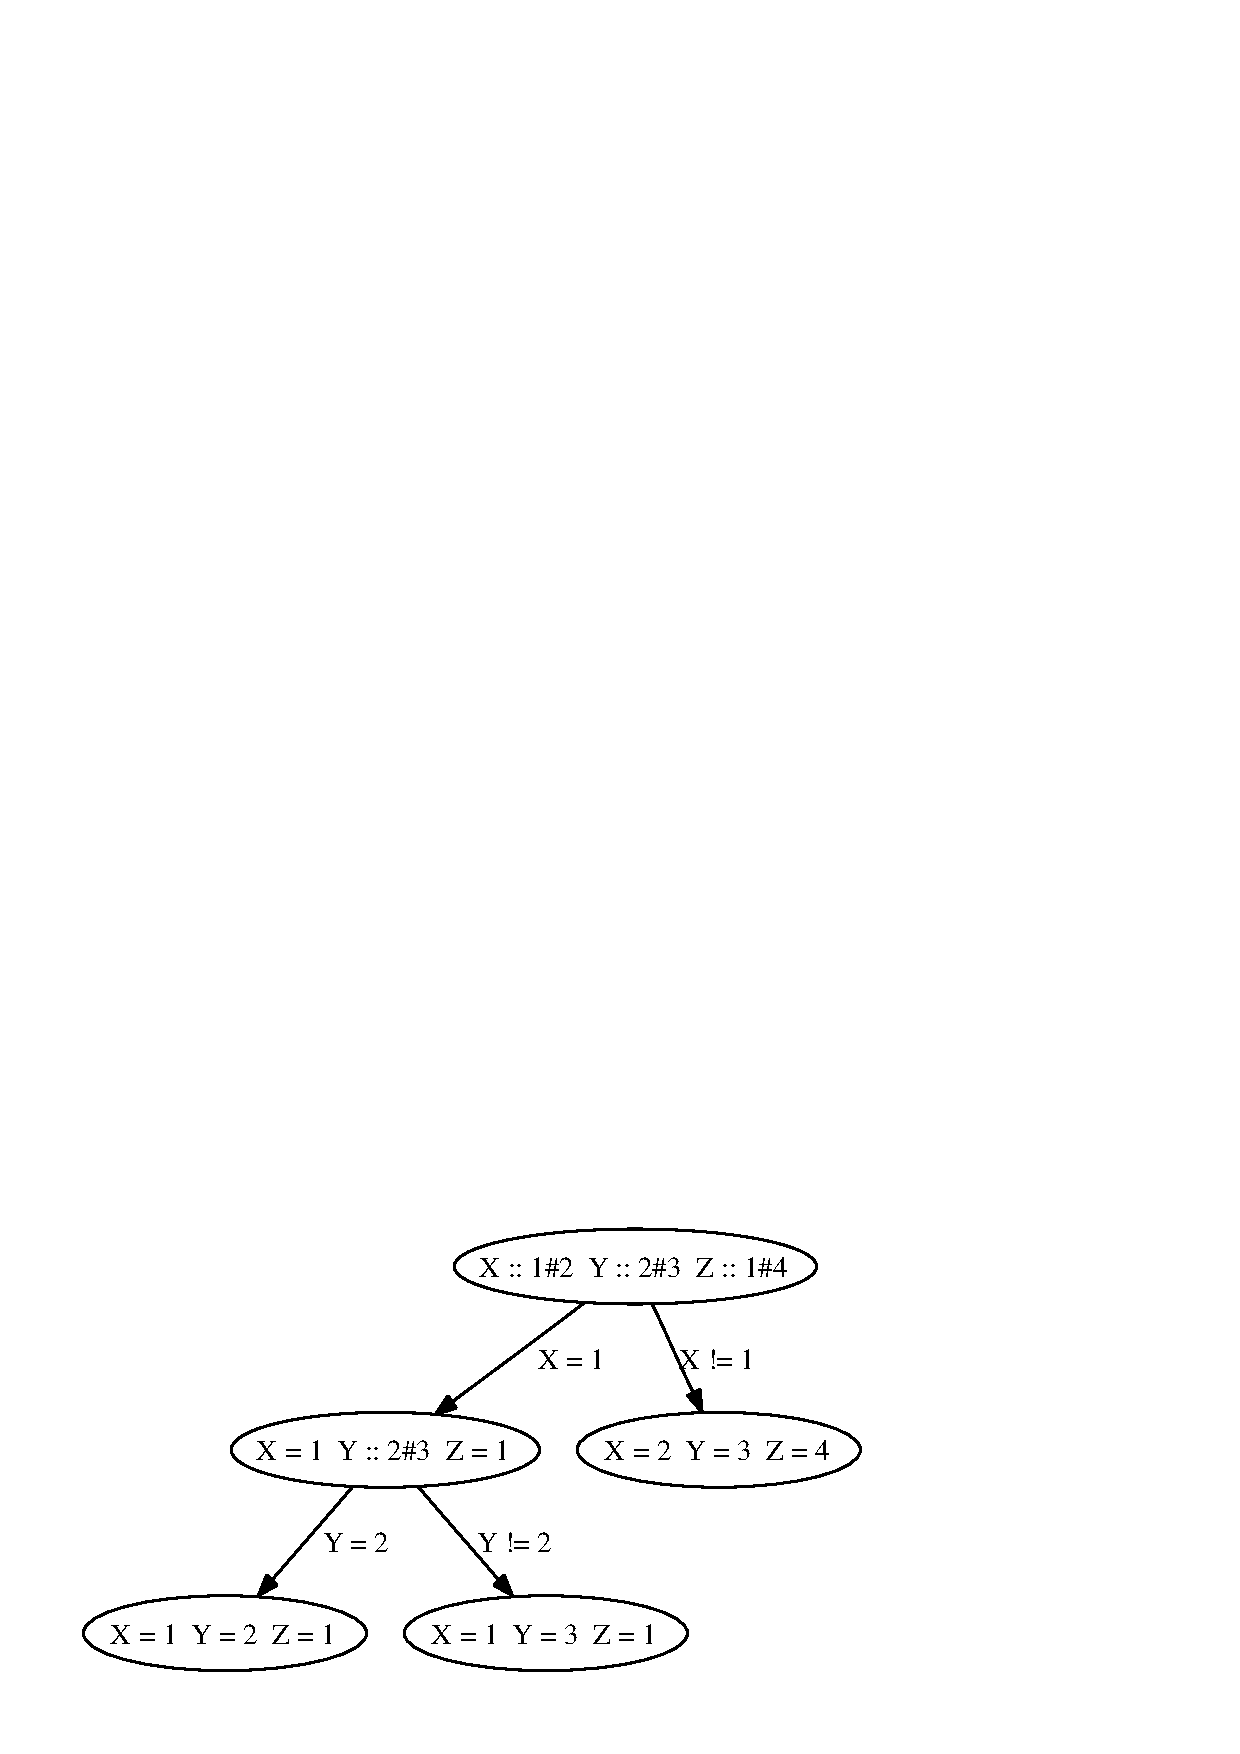
\includegraphics[height=6cm]{../images/searchtree-values} 
  } \subfloat[Suchbaum als Graph]{
    \label{fig:distribuierung-suchbaum-2}
  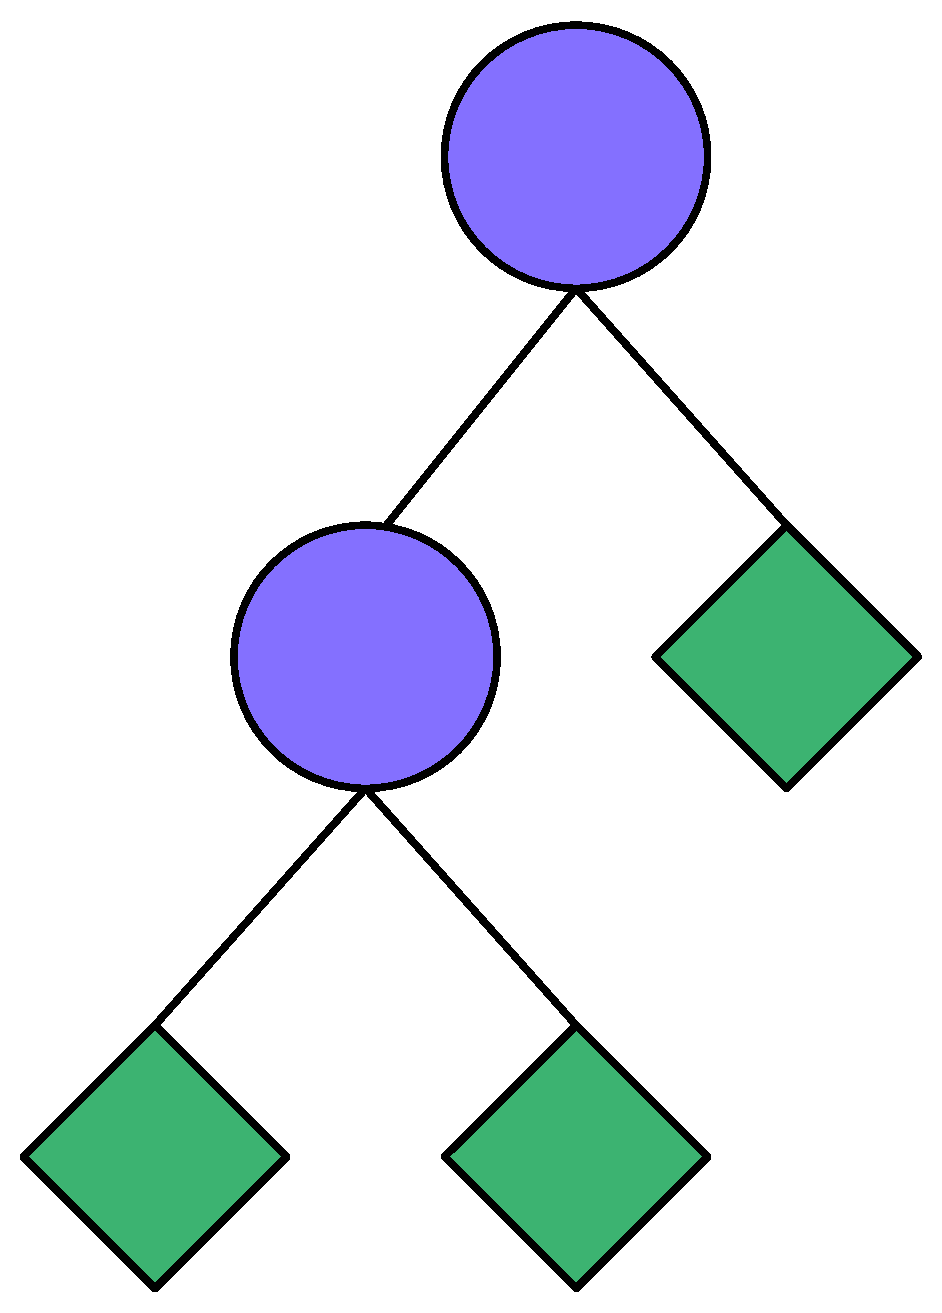
\includegraphics[height=6cm]{../images/searchtree-graph} 
  }
  \caption{Distribuierung}
  \label{fig:distribuierung-suchbaum}
\end{figure}

\subsection{Beispiel "`Send More Money"'}
Nachfolgend möchten wir anhand eines konkreten Beispiels die 
Wissensverarbeitung mithilfe der Constraint Programmierung in Oz demonstrieren. 
Entnommen ist diese Lösung des "`Send More Money"'-Problems der 
Mozart-Dokumentation \cite[Finite Domain Constraint Programming in
  Oz, Chapter 3.2]{url:mozart-documentation}.

\subsubsection{Problemdefinition und Modell}
Gegeben sei die Gleichung $$SEND + MORE = MONEY$$ Ziel ist es, den einzelnen
Buchstaben paarweise verschiedene Ziffern zwischen 0 und 9 zuzuweisen. Außerdem
soll gelten: $S \neq 0$ und $M \neq 0$.

\subsubsection{Programm}
Listing \ref{lst:sendMoreMoney} zeigt den Quellcode des fertigen Oz-Scripts.

\lstinputlisting[label={lst:sendMoreMoney}, caption={Das "`Send More 
Money"'-Problem in Oz}]{../sendMoreMoney.oz}

Es werden zunächst für alle Buchstaben Variablen deklariert und anschließend ein
\texttt{Record} angelegt, der für jeden Buchstaben einen Eintrag enthält (Zeile
6). In den nachfolgenden Zeilen werden die einzelnen Constraints deklariert: 

\begin{itemize}
  \item alle Einträge in \texttt{Root} sind beschränkt auf $(0, 9)$,
  \item alle Einträge in \texttt{Root} sind paarweise verschieden (distinct),
  \item S und M sind ungleich 0,
  \item die Werte der einzelnen Buchstaben erfüllen die Gleichung.
\end{itemize}

In Zeile 14 wird die Distribuierung mit der sog. "`first-fail"'-Strategie 
angestoßen. Bei dieser Strategie wird zur Erzeugung des zur Distribuierung
benötigten Constraints die höchstwertige Variable verwendet, bei der die Anzahl
möglicher Werte minimal ist.

Schließlich wird in Zeile 17 die Suche nach der Lösung begonnen (s. Kapitel 
\ref{subsection:Search}) und in der darauf folgenden Zeile der Suchbaum 
ausgegeben.

\subsection{Beispiel Sudoku}
Anhand eines weiteren Beispiels möchten wir die Lösung von Problemen und die 
Wissensverarbeitung in Oz zeigen. Sudoku ist ein Logikrätsel, das sich in den 
letzten Jahren großer Beliebtheit erfreut hat. In der Regel besteht ein 
Sudoku-Rätsel aus einem $9 \times 9$-Gitter, das mit einigen Zahlen vorbelegt 
ist. Ziel ist es, die freien Felder des Gitters so zu füllen, dass in der jeder 
\textsl{Reihen}, \textsl{Spalten} und in jedem der neun \textsl{$3 \times 
3$-Unterquadrate} die Ziffern zwischen 1 und 9 genau einmal vorkommen.

Abbildung \ref{fig:sudoku-beispiel} zeigt ein Beispiel für ein Sudoku-Rätsel im
Startzustand.

\begin{figure}[hp]
	\begin{sudoku}
	| |1|2| | |9|6| | |.
	| | |7|3|5| | |9| |.
	|8| | | |4| | |3|7|.
	|4| |3|2| | | |1| |.
	| |8| |7|6| |9| | |.
	|9| | | | |3|8| |4|.
	| |6| | | |5|7| |1|.
	|7| |9|6| |1| | | |.
	| |5| | |2| | |6|9|.
	\end{sudoku}
  \caption{Ein $9 \times 9$-Sudoku}
  \label{fig:sudoku-beispiel}
\end{figure}

\subsubsection{Problemdefinition und Modell}

Gegeben sei ein Sudoku Quadrat der Ordnung $n$, das ein $n^2 \times n^2$-Gitter 
mit $n^4$ Felder mit den Werten von $0$ bis $n^2$ bildet 
\cite{sudoku-as-constraint}. Jeder Wert, $0$ bis $n^2$, darf in jeder Reihe, 
jeder Spalte und in jedem der $n^2$ $n \times n$-Unterquadrate genau einmal 
vorkommen.

Üblicherweise werden Sudokus der Ordnung $3$ ($9 \times 9$-Gitter) verwendet.
Laut \cite{sudoku-as-constraint} gibt es 6.670.903.752.021.072.936.960 komplett
ausgefüllte und gültige Sudoku-Quadrate der Ordnung $3$.


Darstellen lässt sich das Sudoku-Problem (hier: $9 \times 9$-Sudoku) auch als
Graphfärbeproblem, wie Abbildung \ref{fig:sudoku-graph} zeigt.

\begin{figure}
  \centering
  \def\JPicScale{0.5}
  \input{../images/sudoku-graph.pst}
  \caption{Linker oberer Block eines Sudoku-Rätsels als Graph}
  \label{fig:sudoku-graph}
\end{figure}

Aus diesem Graphen lässt sich direkt ableiten, wann ein Knoten mit einem anderen
Knoten durch eine Kante verbunden ist. Dies ist genau dann der Fall, wenn

\begin{itemize}
  \item $x = x'$, (Knoten liegen in derselben \textsl{Spalte}) oder
  \item $y = y'$, (Knoten liegen in derselben \textsl{Zeile}) oder
  \item $\left\lceil \nicefrac{x}{3} \right\rceil = \left\lceil
  \nicefrac{x'}{3} \right\rceil \wedge \left\lceil \nicefrac{y}{3} \right\rceil
  = \left\lceil \nicefrac{y'}{3} \right\rceil$ (Knoten liegen im selben
  $3 \times 3$-Block).
\end{itemize}

Das Problem besteht nun darin, dass benachbarte Knoten nicht den selben Ziffen
(analog: Farben) zugeordnet werden dürfen. Es lassen sich also die folgenden $3
\cdot 9 = 27$ Constraints ableiten:

\begin{itemize}
  \item \textsl{distinct((0,0), (1,0), \ldots, (8,0))} (Zeile 1)
  \item \textsl{distinct((0,1), (1,1), \ldots, (8,1))} (Zeile 2)
  \item \ldots
  \item \textsl{distinct((0,0), (0,1), \ldots, (0,8))} (Spalte 1)
  \item \textsl{distinct((1,0), (1,1), \ldots, (1,8))} (Spalte 2)
  \item \ldots
  \item \textsl{distinct((0,0), (1,0), \ldots, (2,2))} (Block 1)
  \item \textsl{distinct((3,0), (4,0), \ldots, (2,5))} (Block 2)
  \item \ldots
\end{itemize}

Es ergibt sich also für jede Zeile, jede Spalte und jede Block-Zelle ein
Constraint. 

\subsubsection{Programm}
Listing \ref{lst:sudoku-solver} zeigt unser erstelltes Programm zur Lösung eines
$3 \times 3$-Sudokus.

\lstinputlisting[label={lst:sudoku-solver}, caption={Lösen eines Sudoku-Rätsels
mit Mozart}, firstline=11, lastline=65, mathescape=false]{../sudokuSolver.oz}

Wir bilden zunächst in der Prozedur \texttt{ErstelleFeld} mithilfe eines 
Records die 81 Zellen in einer Datenstruktur ab, um diesen Variablen später die 
Constraints zuweisen zu können. Außerdem wird dort die Vorbelegung des Feldes
getätigt, wir verwenden hier das Beispiel aus Abbildung
\ref{fig:sudoku-beispiel}.

Der Prozedur \texttt{Sudoku} wird ein Feld übergeben und es wird anschließend 
durch Erstellen der erwähnten Constraints die Lösung des Rätsels ermittelt. 
Dieses wird in der Variablen \texttt{Loesung} abgelegt. Wie man sieht, wird für 
die Lösung dieses Sudokus keine Distribuierung benötigt, da sich die Lösung 
allein durch die Auswertung der Constraints ergibt! Schließlich können wir die 
Lösung graphisch ausgeben. Aus Platzgründen ist dieser Teil des Quellcodes hier 
nicht aufgeführt, er findet sich im Anhang in Listing 
\ref{lst:sudoku-solver-gui}. Abbildung \ref{fig:sudoku-solver} zeigt die 
Oberfläche des Sudoku-Lösers, mit dem in Abbildung \ref{fig:sudoku-beispiel} 
vorgestellten Beispiel für ein Sudoku. Das Sudoku kann über einen Klick auf den 
Button "`Lösen"' gelöst werden. Das korrekt ausgefüllte Sudoku ist in Abbildung 
\ref{fig:sudoku-solved} zu sehen.

\begin{figure}
   \centering
   \subfloat[Ungelöstes Sudoku]
   {
     \label{fig:sudoku-unsolved}
     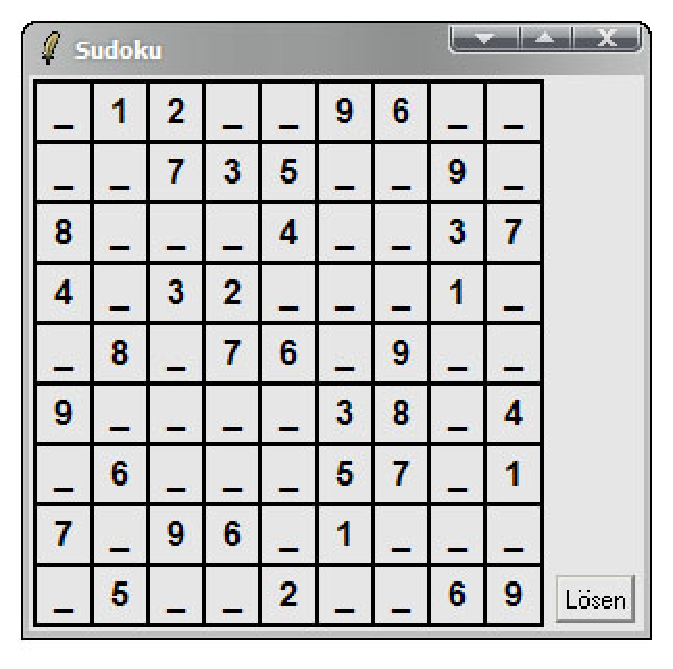
\includegraphics[width=0.4\textwidth]{../images/sudoku-unsolved}
   } 
   \subfloat[Gelöst]
   {
     \label{fig:sudoku-solved}
     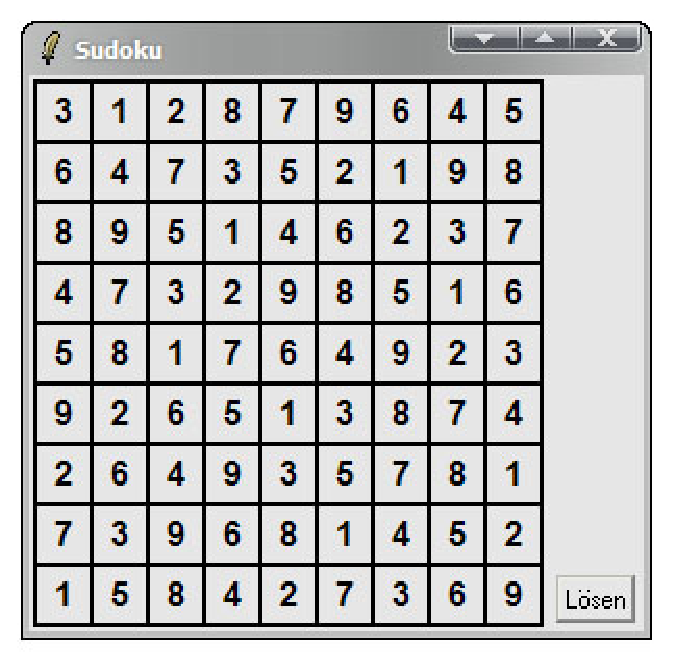
\includegraphics[width=0.4\textwidth]{../images/sudoku-solved}
   }
   \caption{Oberfläche des Sudoku-Lösers}
   \label{fig:sudoku-solver}
\end{figure}

\section{Funktionale Programmierung}
Die funktionale Programmierung fußt auf der Auswertung (mathematischer)
Ausdrücke. Funktionen verhalten sich hierbei - im Gegensatz zu anderen,
nicht-funktionalen Programmiersprachen - wie mathematische Funktionen. Dies hat
u.a. den Vorteil, dass Programme sich nun mit mathematischen Beweisverfahren
besser validieren lassen. Ein wichtiges Merkmal funktionaler Programme ist, dass
anstatt Schleifen und Zuweisungen mit Rekursion gearbeitet wird.

Oz unterstützt sowohl die sog. \textsl{eager evaluation} als auch
\textsl{lazy evaluation}. Eager evaluation (strikte Auswertung) bedeutet, dass
Argumente einer Funktion vor Ausführung der eigentlichen Funktion ausgewertet
werden. Im Gegensatz dazu werden Argumente bei der lazy evaluation erst bei
Bedarf ausgewertet, also dann, wenn deren Wert in einer Rechenoperation benötigt
wird.

Listing \ref{lst:mapEager} zeigt ein einfaches Beispiel für funktionale
Programmierung in Oz.

\lstinputlisting[label={lst:mapEager}, mathescape=false,
caption={Funktionales Programm mit eager evaluation}]{../mapEager.oz}

Der Funktion \texttt{Map} wird eine Liste sowie eine Funktion übergeben; die 
Funktion wird dann rekursiv auf alle Listenelemente angewandt. In Zeile 9 wird 
\texttt{Map} beispielhaft mit der Liste \texttt{[1 2 3 4]} und einer anonym 
definierten Funktion aufgerufen.

\section{Objektorientierte Programmierung}
Mit Einführung der Programmiersprache Smalltalk hat die objektorientierte 
Programmierung weite Verbreitung gefunden und ist heutzutage das in der 
Wirtschaft am häufigst eingesetzten Programmierparadigma. Objekte kapseln 
(veränderlichen) \textsl{Zustand} und \textsl{Verhalten}. Besonders in 
Anwendungen, die mit externen Systemen oder Anwendern interagieren eignen sich 
Objekte gut, um die Problemstellung imperativ zu formulieren und zu lösen 
\cite{KI-LP96}.

In Oz lassen sich Klassen mit Attributen und Methoden deklarieren und 
anschließend Objekte dieser Klassen erzeugen. Weiterhin kann der Anwender seine
Klassenhierarchie mit Mehrfachvererbung aufbauen. Listing \ref{lst:counter}
zeigt die Deklaration einer Klasse \texttt{Counter} sowie einige
Methodenaufrufe. 

\lstinputlisting[label={lst:counter}, mathescape=false,
caption={Deklaration einer Klasse und Erzeugen eines Objekts}]{../counter.oz}

In Zeile 16 wird ein Objekt der Klasse \texttt{Counter} erzeugt und der
Variablen \texttt{C} zugewiesen. Die Zeilen 17 und 18 zeigen Aufrufe der
Methoden \texttt{inc()} bzw. \texttt{browse()}.

\section{Logische Programmierung}
Mithilfe von logischen Programmiersprachen wie z.B. Prolog lassen sich Probleme
lösen, für die kein (effizienter) Algorithmus bekannt ist, man also nach der
Lösung \textsl{suchen} muss. Diese Art von Problem taucht bspw. in der
Künstlichen Intelligenz, der Sprachverarbeitung oder der Unternehmensforschung
(Operation Research) auf \cite[Tutorial of Oz,
Chapter 12]{url:mozart-documentation}.

Oz erweitert die Ideen von Prolog und setzt dabei nicht auf die von Prolog
bekannten Horn-Klauseln, sondern verwendet eine einfache Kompositions-Syntax
höherer Ordnung \cite{LogicProgr:2003}. 

Mithilfe der logischen Programmierung lassen sich aber nicht nur die genannten 
Suchprobleme lösen, sondern auch herkömmliche algorithmisch lösbare Probleme.
Listing \ref{lst:detAppend} zeigt zunächst ein \textsl{deterministisches}
Programm, d.h. es ist keine Suche nötig.

\lstinputlisting[label={lst:detAppend}, mathescape=false,
caption={Deterministisches logisches Programm}]{../detAppend.oz}

Die Funktion \texttt{Append} soll den übergebenen Parameter \texttt{Ys} an 
\texttt{Xs} anhängen und das Ergebnis zurückliefern. In Zeile 8 wird in dem 
beispielhaften Aufruf \texttt{X} an die Liste \texttt{[1 23 abc]} angehängt.

Im Gegensatz dazu wird bei der \textsl{nicht-deterministischen} Programmierung
davon ausgegangen, dass man nur durch Suche die bzw. alle Lösungen finden kann.
In Oz lässt sich so etwas mithilfe des \texttt{choice}-Statements realisieren,
wie Listing \ref{lst:nonDetAppend} zeigt.

\lstinputlisting[label={lst:nonDetAppend}, mathescape=false, 
caption={Nicht-deterministisches logisches Programm. Quelle: 
\cite{LogicProgr:2003}}]{../nonDetAppend.oz}

Hier wird zunächst wieder die Prozedur \texttt{Append} definiert, dieses mal
jedoch wird ein sog. \textsl{choice-point} festgelegt. Anschließend wird eine
weitere Prozedur \texttt{Anfrage} deklariert, welche die Suchanfrage beinhaltet
und das Ergebnis zurückliefert. Die eigentliche Suche wird über die Klasse
\texttt{Search} (s. auch Kapitel \ref{subsection:Search}) verwaltet. Über die
Methode \texttt{next()} (Zeile 21) lässt sich die jeweils nächste Lösung
ermitteln - auf diese Weise können sukzessive alle Lösungen bestimmt werden.

 
\section{System Module}
Neben der Implementierung der Basisumgebung für Oz bietet das Mozart Programming
System auch so genannte \textsl{System Module}, die ein effektiveres und
effizienteres Entwickeln von Anwendungen ermöglichen. Die Module lassen sich in
mehrere Einsatzgebiete gliedern, die im Folgenden erläutert werden. 
 
\section{Application Programming}

Für das \textsl{Application Programming} finden sich zwei Module, die das
Arbeiten mit Applikationen und das Verwenden der vorhandenen Module erleichtern.

\begin{description}
  \item[\texttt{Application}] Das Modul \texttt{Application} ermöglicht den
  Zugriff auf die Argumente einer Anwendung und bietet Prozeduren um
  Anwendungen zu beenden. Der Zugriff auf die Argumente ist vergleichbar mit
  \texttt{Strings[] args} in Java. Es stehen 3 verschiedene Argumentarten für
  Web-, Kommandozeilen- und GUI-Anwendungen zur Verfügung. Außerdem können mit
  Hilfe dieses Moduls die Argumente auf unterschiedliche Arten geparst und
  verarbeitet werden. 
  \item[\texttt{Module}] Für den Zugriff, das Linken und Laden von Modulen ist
  das Modul \texttt{Module} zuständig. Hier kann auf vorhandene Module, wie z.B.
  \texttt{Application}, zugriffen werden um Prozeduren zu verwenden. Außerdem
  können eigene Oz-Anwendungen als Module geladen werden und später dann gelinkt
  werden.
\end{description}

\section{Constraint Programming}

Die Module, die in den Bereich des \textsl{Constraint Programming} fallen,
stellen einen der wichtigsten Teile für die Erweiterung von Oz dar. Hier finden
sich Module, die die Semantik und Syntax für das Constraint Programming
erweitern. Beispielsweise wird die Semantik durch das Modul \texttt{FD} um
\textsl{Finite Set Constraints} erweitert, eine Erweiterung auf Mengen von
Constraints. 

Ein kurzer Überblick aller Module für das Constraint Programming,
\begin{description}
  \item[\texttt{Search}] Dieses Modul bietet Unterstützung für die \textsl{Suche} von
  Lösungen, näheres siehe Punkt \ref{subsection:Search}. 
  
  \item[\texttt{FD}] Für den leichteren Umgang mit \textit{Finite Domain Constraints}
  finden sich in diesem Module beispielsweise vordefinierte Propagatoren, siehe
  Punkt \ref{subsection:FD}.
  
  \item[\texttt{Schedule}] Das Modul \texttt{Schedule} unterstützt die
  Entwicklung von Scheduling-Anwendung\-en, in denen Tasks auf gegebene Ressourcen
  verteilt werden, so dass keine zeitlichen Überlappungen auftreten. In
  \cite[System Modules, Part II]{url:mozart-documentation} wird diese
  Vermeidung von zeitlichen
  Überlappungen als \textsl{Serialization for Unary Resources} bezeichnet.
  Außerdem bietet das Modul Propagatoren und Verteiler um mehrere Tasks, die
  verschiedene Ressourcen benötigen, so zu verteilen, damit jede Ressource
  \textsl{serialized} ist. Zusätzlich wird auch noch das so genannte kumulative
  Scheduling unterstützt, hier dürfen die Kapazitäten der Ressourcen nicht
  überschritten werden.
  
  \item[\texttt{FS}] Hinter diesem Modul verbergen sich \textsl{Finite Set
  Constraints}. Es handelt sich um eine neue Constraint-Art für Oz, die eine
  $n$-elementige Menge mit $n$ finite Domain Variablen assoziiert. Mengen von
  Constraint Variablen erweisen sich, laut \cite[System Modules, Part
  II]{url:mozart-documentation}, bei
  kombinatorischer Suche und Natural Language Processing als sehr nützlich. Im
  Umfang des Moduls befinden sich Prozeduren, Propagatoren etc. für den
  einfachen Umgang mit Finite Set Constraints.
  
  \item[\texttt{RecordC}] Um auch mit anderen Datentypen als Domain Variablen,
  Intervall von Integern, auf den Constraint Store zuzugreifen, bietet das
  Modul \texttt{RecordC} die Möglichkeit, Constraints vom Datentyp
  \texttt{Record} zu verwenden. Es werden Prozeduren angeboten um das
  \textsl{Telling} auf den Store für Records zu erweitern.
  
  \item[\texttt{Combinator}] Damit Constraints miteinander kombiniert werden
  können, bietet dieses Modul Prozeduren zur Kombination der Constraints. Bei den
  Kombinatoren handelt es sich hauptsächlich um konditionale oder logische, wie
  z.B. \texttt{Combinator.'or'} oder \texttt{Combinator.'not'}. Hier handelt
  sich um eine direkte Erweiterung der Oz-Syntax, die ohne weiteren Aufwand
  verwendet werden kann, daher werden die Operatoren auch als String aufgerufen.
  
  \item[\texttt{Space}] Mit Hilfe dieses Moduls können eigene \textsl{Inferenzmaschinen}
  erstellt werden. Es werden Prozeduren bereitgestellt, mit denen Spaces
  verwaltet werden können. Durch die eigene Verwaltung, wie das Erzeugen neues
  Spaces \texttt{Spaces.create} oder das Zusammenfügen von Spaces
  \texttt{Spaces.merge}, können für die Inferenzmaschine neue Schlussfolgerungen
  erreicht werden. 
\end{description}

Im Folgenden wird näher auf die Module \texttt{Search} und \texttt{FD} 
eingegangen, da diese den meisten Einsatz beim Constraint Programming finden.

\subsection{Modul \texttt{Search}}
\label{subsection:Search}

Für die Suche bietet das Modul 3 Möglichkeiten, die
\textsl{Basis-Suchmaschinen}, die \textsl{Universellen Suchmaschinen} und die
\textsl{Parallele Suche}. Allgemein ist zur Suche in Mozart zu sagen, dass nach
einer bzw. der ersten möglichen Lösung, allen Lösungen und der besten Lösung
gesucht werden kann. Für die Suche nach der besten Lösung muss noch eine Ordnung
übergeben werden, die definiert, was eine gute oder schlechte Lösung ist.

\subsubsection{Basis-Suchmaschinen}

Um die Suche mit den Basis-Suchmaschinen zu ermöglichen, müssen in den
Prozeduren, mit denen eine Lösung gefunden werden soll, Entscheidungspunkte 
gesetzt werden. Dieses Setzten der Punkte erfolgt über das Schlüsselwort
\texttt{choice}, das nebenbei bemerkt aus dem Modul \texttt{Combinator} stammt. 

Ein kleines Beispiel nach \cite{LogicProgr:2003} zur Verdeutlichung. Hier sollen
nach den Kinder eines gegebenen Vaters gesucht werden.

\lstinputlisting[
	mathescape=false,
	caption={Suche nach allen Lösungen}, 
	label={lst:baseSearch}]
	{../baseSearch.oz} 

Der letzte Aufruf in Listing \ref{lst:baseSearch} stößt die Suche mit dem Vater
"`terach"' an. Durch den Aufruf \texttt{Search.base.all} wird nach allen
möglichen Lösungen gesucht und als Ergebnis wird die Liste \texttt{[abraham
nachor haran]} zurückgegeben.

\subsubsection{Universelle Suchmaschinen}

Mit den Universellen Suchmaschinen lässt sich eine parametrisierte Suche
durchführen. Hierzu bietet das Modul die Möglichkeit des so genannten
\textsl{Recomputation} \cite[System Modules, Part II, Chapter
4.2]{url:mozart-documentation}, die Suche zu stoppen
und verschiedene Ausgabemodi zu verwenden.

Mit Hilfe des Recomputation können auch für sehr große Suchbäume, für die in der
Regel nicht genügend Speicherplatz zur Verfügung steht, Lösungen gefunden
werden. Bei der normalen Suche in Oz wird in jedem Distributionschritt eine
neue Kopie des Spaces erstellt. Dadurch kann der Speicherbedarf bei sehr großen
Suchbäumen schnell sehr groß werden. Um diesem Problem Abhilfe zu schaffen, kann
mittels der Recomputation angegeben werden, dass nur alle $n$ Distributionsschritte
eine Kopie erstellt werden soll. Die Verringerung des Speicherbedarfs geht
allerdings auf die Kosten der Zeit. Schlägt eine Suche im $n-1$-ten Schritt nach
der letzten Kopie fehl, muss zur letzten Kopie zurück gesprungen werden und
einige Suchpfadteile könnten mehrfach durchsucht werden.

\subsubsection{Parallele Suche}

Mit Hilfe der parallelen Suche soll die Exploration von Suchbäumen beschleunigt
werden, siehe \cite[System Modules, Part II, Chapter
4.4]{url:mozart-documentation}. Um die Suche zu parallelisieren,
wird der Suchbaum in mehrer Untersuchbäume aufgeteilt und auf mehrere
Oz-Prozesse verteilt. Die Verteilung auf mehrere Oz-Prozesse kann lokal auf
einen PC laufen oder auch auf mehrere PCs im Netzwerk verteilt werden. Damit die
Suche parallel laufen kann, stellt das Modul die Klasse \texttt{Search.parallel}
bereit, die alle Aufgaben übernimmt.

\subsection{Finite Domain Constraints: \texttt{FD}}
\label{subsection:FD}

Ein weiterer wichtiger Teil für das Constraint Programming stellt das Modul
\texttt{FD} für \textsl{Finite Domain Constraints} dar. Das Modul definiert
Prozeduren, Propagatoren und Distributions-Strategien für die Suche.

Die meisten hier definierten Prozeduren und Propagatoren können implizit in Oz
verwendet werden. Beispielsweise bedarf es bei Prozeduren für das Telling auf den
Constraintstore keinen expliziten Import des Moduls. Die definierten
Propagatoren gliedern sich in generische, symbolische, und binäre (0/1
Propagatoren), vgl. \cite[System Modules, Part II, Chapter 5
]{url:mozart-documentation}. Die generischen
Propagatoren lassen Definitionen für den Wertebereich von Domain Variablen zu,
z.B. kleiner gleich "`\texttt{=<:}"', die auch implizit in Oz verwendet werden
können. 

Zusätzlich bietet das Modul \textsl{Reflection} und das so genannte
\textsl{Watching}, nach \cite[System Modules, Part II, Chapter
5.5]{url:mozart-documentation}, für Domains (Domain
Variablen) an. Bei Reflection kann z.B. die aktuelle untere oder obere Grenze
der Domain Variable zurückgegeben werden, \texttt{reflect.min} bzw.
\texttt{reflect. max}. Mittels des Watching können Domains beobachtet werden.
Beispielsweise wird \texttt{true} bei \texttt{\{FD.watch.size *Domain1 +Domain2
?B\}} zurück gegeben, wenn die Intervallgröße von \texttt{Domain1} kleiner
wird als die Größe von \texttt{Domain2}.

\section{Verteilte Programmierung}

Für die Entwicklung von \textsl{verteilten Anwendungen} bietet das Mozart
Programming System einen Satz von Modulen, die die Entwicklung erleichtern.
Neben Modulen für den Verbindungsaufbau oder die Remote-Steuerung von
Oz-Prozessen, finden sich auch Module für die Manipulation für URLs (Uniform
Resource Locator) oder für statistische Analysen der Verteilung.

Ein Überblick aller verfügbaren Module für die verteilte Programmierung, 

\begin{description}
  \item[\texttt{Connection}] Um in Oz eine Verbindung zwischen Oz-Prozessen
  herzustellen, werden so genannte \textsl{Tickets}
  \cite[System Modules, Part III]{url:mozart-documentation} verwendet. Ein
  Ticket stellt einen String
  dar, der für den Verbindungsaufbau verschickt wird. Um eine Verbindung
  herzustellen, erzeugt ein Prozess, der so genannte \textsl{Server}, ein Ticket,
  das vom \textsl{Client} auf der anderen Seite geholt bzw. empfangen wird.
  Das Modul \texttt{Connection} unterscheidet hier zwei Verbindungstypen,
  nach \cite[System Modules, Part III]{url:mozart-documentation}:
  \begin{description}
    \item[One-to-one] Erlaubt nur Einzelverbindungen zwischen 2 Prozessen, mit
    einem einmal verwendbaren Ticket.
    \item[Many-to-one] Erlaubt Verbindung von mehreren Clients zu einem Server
    mit dem gleichen Ticket.
  \end{description}
  \item[\texttt{Remote}] Mittels dieses Moduls können über das Netzwerk andere
  Oz-Prozesse gestartet werden. Diese neu erzeugten Prozesse können
  \textsl{remote} gesteuert werden. Von der Klasse \texttt{Remote.manager} wird
  auf einem Computer im Netzwerk eine Instanz erzeugt, der so genannte
  \textsl{Remote Modul Manager}, der es erlaubt remote den Prozess zu steuern
  und auf die Ressourcen des entfernten Computers zuzugreifen. 
  \item[\texttt{URL}] Das Modul \texttt{URL} dient zur Erzeugung und Manipulation
  von URLs, für das WWW und das Dateisystem. Durch die Prozedur \texttt{URL.make}
  wird eine URL erzeugt, die sich als Datenstruktur verwalten lässt,
  beispielsweise \texttt{\{URL.make 
  "'http://www. mozart\-oz.org/home-1.1.0/share/FD.ozf"'\}}. Das Modul kümmert
  sich um die systemspezifischen Seperatoren für Verzeichnisse, somit spielt es
  keine Rolle, ob Verzeichnisse durch \verb+\+ oder \verb+/+ getrennt werden.
  
  \item[\texttt{Resolve}] Damit schnell Dateien oder Unterverzeichnisse in
  einer URL gefunden und verarbeitet werden können, bietet das Modul
  \texttt{Resolve} einige Prozeduren. Wie der Name schon sagt, soll die
  übergebene URL nach verschiedenen Arten aufgelöst werden, z.B. kann mit
  \texttt{root} das Rootverzeichnis für alle übergebenen URLs gesetzt werden.
  
  \item[\texttt{Fault}] Mit Hilfe dieses Moduls können Fehler bei Verteilung
  erkannt und behandelt werden. Anzumerken ist an dieser Stelle, dass dieses
  Modul laut der Dokumentation \cite[System Modules, Part
  III]{url:mozart-documentation} im aktuellen
  Release (Version 1.3.2) noch nicht komplett fertig gestellt ist.
  
  \item[\texttt{Discovery}] Bei der Lokation von Diensten (Oz-Servern) im
  Netzwerk hilft das Modul \texttt{Discovery}. Ein Oz-Server wird im einen Wert
  initialisiert, in der Regel mit einen Ticket, und wartet bis ein Client eine
  Anfrage startet. Sucht ein Client einen Dienst im Netzwerk sendet er einen
  Broadcast über das Netzwerk und wartet auf die Antwort des zugehörigen
  Servers. In der aktuellen Version 1.3.2 ist die Funktionalität nur für Linux-
  und Solaris-Netzwerke verfügbar, siehe \cite[System Modules, Part
  III]{url:mozart-documentation}. 
  
  \item[\texttt{DPInint}] Die so genannte Verteilungsschicht, nach
  \cite[System Modules, Part III]{url:mozart-documentation}, wird bei Mozart nur
  bei Bedarf dynamisch
  nachgeladen. Über das Modul \texttt{DPInit} können einige Parameter zur
  Ladezeit der Verteilungsschicht initialisiert werden. \texttt{IpPort} legt
  beispielsweise fest über welchen Port kommuniziert werden soll. 
  
  \item[\texttt{DPStatistics}] Das Modul \texttt{DPStatistics} unterstützt die
  statistische Analyse von verteilten Anwendungen, um möglicherweise einige
  Aspekte verbessern zu können. Mit Hilfe des Moduls können Logfiles in
  verschiedenen Ausgabemodi erstellt werden. 
\end{description}

\section{Open Programming}

In der Mozart Dokumentation \cite[System Modules, Part
IV]{url:mozart-documentation}  werden diese Module
als Verbindung zum Rest der \textsl{Computational World} beschrieben. Mit Hilfe
dieser Module erhält man Zugriff auf Dateien und Zugang zum Betriebssystem.

\begin{description}
  \item[\texttt{Open}] Mit diesem Modul ermöglicht Mozart den Zugriff auf
  Dateien (\texttt{Open.file}), Sockets (\texttt{Open.socket}) und Pipes
  (\texttt{Open.pipe}). Wie üblich können Dateien geöffnet, eingelesen,
  geschrieben und wieder geschlossen werden. Mit Sockets können Verbindungen zum
  Netzwerk über TCP oder UDP geöffnet und verarbeitet werden. Über die Klasse
  \texttt{Open.pipe} können Prozesse über die übergebene PID (Process ID)
  \textsl{geforkt} werden, um Daten mit diesem Prozess auszutauschen.
  Zusätzlich beinhaltet das Modul die Klasse \texttt{Open.text}, die in
  Verbindung mit den anderen Klassen verwendet werden kann um Text buchstaben-
  oder zeilenweise einzulesen. Außerdem werden Exceptions von diesem Modul
  ausgelöst, falls Probleme beim Zugriff auftreten, z.B. \textsl{already closed}.
  
  \item[\texttt{OS}] Die Prozeduren des Moduls \texttt{OS} sind laut
  \cite[System Modules, Part IV]{url:mozart-documentation} zu POSIX (Portable
  Operating System Interface)
  kompatibel. Hauptsächlich handelt es sich um Prozeduren für die Interaktion
  mit dem Betriebssystem, z.B. das Erzeugen von Zufallszahlen (\texttt{OS.rand})
  oder Zugriff auf das Dateisystem (\texttt{OS.tmpnam}, absoluter Pfad zu einer
  neu erzeugten Datei). Außerdem erhält man auch Zugriff auf Verzeichnisse,
  beispielsweise liefert \texttt{OS.getDir} alle Pfade zu Dateien im gegebenen
  Verzeichnis. Zusätzlich bietet das Modul Zugriff auf Sockets, die Systemzeit und
  Umgebungsvariablen. Bei den so genannten \textsl{Low Level Procedures} können
  Angaben über die Lese- oder Schreibberechtigung gemacht werden, z.B. read only
  usw. Zu diesen Prozeduren zählen auch Prozeduren, wie \texttt{OS.kill}, für
  die Prozess-Steuerung, näheres siehe \cite[System Modules, Part IV]{url:mozart-documentation}.
\end{description}

\section{System Programmierung}

In das Gebiet der System Programmierung fallen Module, die die
\textsl{Funktionalität} das Mozart Programming System betreffen. Im Folgendem
einen Überblick dieser Module,

\begin{description}
  \item[\texttt{Pickle}] Das Modul \texttt{Pickle} dient dazu, zustandslose
  Werte zu speichern, also um Peristenz herzustellen. Die Werte können unter
  einem Dateinamen gespeichert und über diesen wieder geladen werden, z.B.
  komprimierte Speicherung \texttt{Pickle.save\-Compressed}.
  
  \item[\texttt{Property}] Um die Parameter der \textsl{Mozart Engine} (Virtual
  Maschine) abzufragen und zu aktualisieren, dient dieses Modul. Hierzu wird
  eine Schnittstelle mit 3 Prozeduren bereitgestellt. Zum Setzten von
  \textsl{Properties} die Prozedur \texttt{Property.put} und für den Zugriff
  auf die Parameter \texttt{Property.get} (nur Lesen des Parameters) und
  \texttt{Property.condGet}. Die Einstellungen können beispielsweise die
  Distribuierung, die Spaces oder den Speichernutzung betreffen, näheres siehe
  \cite[System Modules, Part V]{url:mozart-documentation}.
  
  \item[\texttt{Error}] Damit Fehlermeldungen, in Form von Exceptions, leserlich
  gestaltet werden können, bietet das Modul \texttt{Error} die Möglichkeit die
  Fehler zu formatieren. So genannte \textsl{Error Formatters} können erstellt
  werden, die Aussage über einen speziellen Fehler geben können. Außerdem bietet
  das Modul Prozeduren zur Fehlerbehandlung in einen Fehlerfall, z.B.
  \texttt{Error.printException}. 
  
  \item[\texttt{ErrorFormatters}] Mozart stellt im Modul
  \texttt{ErrorFormatters} schon einige vordefinierte Fehlermeldungen bereit,
  die von \texttt{Error}-Modul verwendet werden und auch selbst verwendet
  werden können. Beispielsweise formatiert \texttt{os} Exceptions und Fehler,
  die von der Schnittstelle zum Betriebssystem hoch kommen.  
  
  \item[\texttt{Finalize}] Mit Hilfe dieses Moduls können in Functors oder
  Klassen gekapselte Daten (Ressourcen) automatisch wieder freigegeben werden,
  falls der Functor oder die Klasse nicht mehr existiert. Hierfür wird in
  \cite[System Modules, Part V]{url:mozart-documentation} ein Beispiel für eine
  Datenbankverbindung, die
  in einer Klasse gekapselt ist, vorgestellt. Falls die Klasse nicht mehr
  benötigt wird, wird die Instanz durch die Garbage Collection zerstört. Bevor
  allerdings die Instanz gelöscht wird, sollte die Datenbankverbindung
  geschlossen werden, diese Aufgabe übernimmt das Modul \texttt{Finalize}.
  
  \item[\texttt{System}] Im Modul \texttt{System} werden Prozeduren
  zusammengefasst, die in Verbindung mit der Mozart Engine stehen. Die meisten
  Prozeduren beziehen sich auf die formatierte Ausgabe von beispielsweise
  Fehler oder einfachen Strings.
\end{description} 

\section{Window Programming}

Wie bei jeder höheren Programmiersprache stellt Mozart Oz Module für die
Oberflächenprogrammierung bereit. Zur Programmierung nutzt Mozart eine
objektorientierte Schnittstelle zu \textsl{Tk} (Toolkit). Ursprünglich entstand
Tk mit der Skriptsprache Tcl \footnote{\url{http://www.tcl.tk/}} (Tool Command
Language) und stellt ein plattformunabhängiges \textsl{Graphical User Interface
Toolkit} dar, siehe \cite{url:tcl-tk}.  

\begin{description}
  \item[\texttt{Tk}] Dieses Modul stellt die Schnittstelle zu Tk dar. Hier
  können Fenster (\texttt{Tk.frame}), so genannte \textsl{Widgets} oder Buttons
  (\texttt{Tk.button}) zu einer Benutzeroberfläche zusammengestellt werden.
  Außerdem können Bilder zu Darstellung geladen werden. Zusätzlich bietet das Modul
  noch so genannte \textsl{Listeners}, die den Listener des  
  Java-Oberflächenkonzepts ähneln, um die Oberfläche über bestimmte Ereignisse
  zu benachrichtigen, siehe \cite[System Modules, Part VI]{url:mozart-documentation}. 
  
  \item[\texttt{TkTools}] Um die Erstellung von Oberflächen zu erleichtern, wird
  das Modul \texttt{TkTools} von Mozart bereitgestellt. In diesem Modul finden
  sich vordefinierte Oberflächenkomponenten, wie Dialoge
  (\texttt{TkTools.dialog}) oder Menüleisten (\texttt{TkTools.menubar}), die
  einfach in der GUI verwendet werden können.
\end{description}

 

\section{Projekte und aktuelle Entwicklungen}
Schließlich noch 2 kurze Beispiele was in Form von Projekten rund um Mozart und
Oz passiert. Zunächst wird ein sehr interessantes Projekt, \textsl{Strasheela},
vorgestellt, das sich mit dem regelbasierten Komponieren von Musik beschäftigt.
Außerdem wird kurz auf einen Versuch eingegangen, bei dem Mozart und Oz in die
Eclipse IDE integriert werden soll. 

\section{Strasheela}

Das von Torsten Anders veröffentliche
\textsl{Strasheela}\footnote{\url{http://strasheela.sourceforge.net/strasheela/doc/}} 
stellt ein in Mozart/Oz implementiertes System dar, mit dem Constraintbasiert
Musik erzeugt werden kann. Der Benutzer gibt deklarativ, in Form von Oz-Code, eine
Musiktheorie an. Oz versucht durch Suche die definierten Constraints zu
terminieren. Um diese Lösungen auch als Musik zu hören, bietet Strasheela die
Möglichkeit die Lösung als MIDI-Datei zu exportieren.

Ein Beispiel, das Strasheela mitliefert, ist sind die so genannten 
\textsl{All-Interval Series}. Diese Musiktheorie stammt aus dem Feld der 
seriellen Musik (serial Musik), siehe \cite{url:serielleMusik}. Eine Serie von 
Tönen besteht in diesem Beispiel aus 12 Tönen einer Tonleiter, die für jede 
Serie nur einmal verwendet werden dürfen. Außerdem müssen die Abstände zwischen 
den einzelnen Tönen eindeutig sein, d.h. pro Serie darf jeder Abstand 
(Intervall) nur einmal vorkommen. Laut \cite{url:strasheela} gibt es für dieses 
Problem 3856 Lösungen, die von Mozart alle gefunden werden, siehe Abbildung 
\ref{fig:strasheela-search}.

\begin{figure}
 \centering
 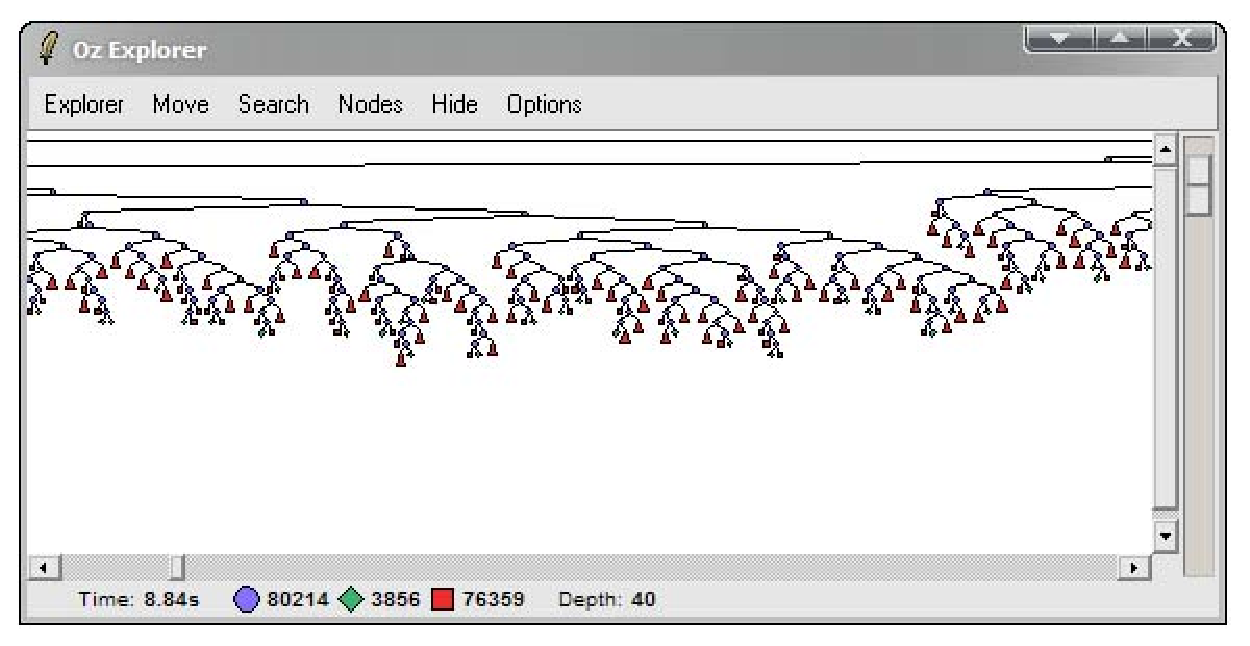
\includegraphics[width=0.6\textwidth]{../images/strasheela-search}
 \caption{Suche nach allen Lösungen von \textsl{All-Interval Series}, grüne
 Raute}
 \label{fig:strasheela-search}
\end{figure}


\section{MozEclipse}

Im Februar diesen Jahres startete Craig Ugoretz das Projekt 
\textsl{MozEclipse}\footnote{\url{http://gforge.info.ucl.ac.be/projects/mozeclipse/}}. 
Ziel dieses Projekts ist es, Mozart und Oz in die Eclipse IDE zu integrieren. 
Durch die Integration soll der Bekanntheitsgrad von Mozart/Oz steigen. Momentan 
ist Mozart in den Emacs integriert, der vor allem Anfängern einige 
Schwierigkeiten bereitet. Durch die Integration in Eclipse sollen die Hemmungen 
beseitigt werden, da viele Anwender gut mit Eclipse vertraut sind. Leider ist 
die Zukunft dieses Projekts noch sehr ungewiss, da es seit dem Anlegen der 
Projekt-Homepage keine weiteren Aktivitäten gab.

% Schluss-Folie
\begin{frame}
  \frametitle{Danke.}
  Fragen?
\end{frame}

\end{document}